\documentclass{article}
\usepackage[T2A]{fontenc} 
\usepackage[utf8]{inputenc} 
\usepackage[english,russian]{babel}
\usepackage{graphicx} 
\usepackage{amsmath}
\usepackage{amsfonts} 
\usepackage{titlesec}
\usepackage{listings}
\usepackage{float}
\usepackage{longtable}
\usepackage{titling} 
\usepackage{geometry} 
\usepackage{pgfplots}
\pgfplotsset{compat=1.9}
\usepackage{xcolor}
\definecolor{darkgreen}{RGB}{0,100,0}

\lstset{
  language=Python,
  basicstyle=\ttfamily,
  keywordstyle=\color{darkgreen},
  stringstyle=\color{purple},
  commentstyle=\color{green},
  morecomment=[l][\color{magenta}]{\#},
  frame=single, 
  showspaces=false, 
  showstringspaces=false, 
  numbers=left, 
  numberstyle=\tiny,
}

\titleformat{\section}
  {\normalfont\Large\bfseries}{\thesection}{1em}{}
\titleformat{\subsection}
  {\normalfont\large\bfseries}{\thesubsection}{1em}{}

\setlength{\droptitle}{-6em} 
\title{Контрольная работа по решению уравнений и систем уравнений}
\author{Винницкая Дина Сергеевна}
\date{Группа: Б9122-02-03-01сцт}

\geometry{a4paper, margin=2cm}

\begin{document}

\maketitle
\begin{figure}[H]
    \centering
    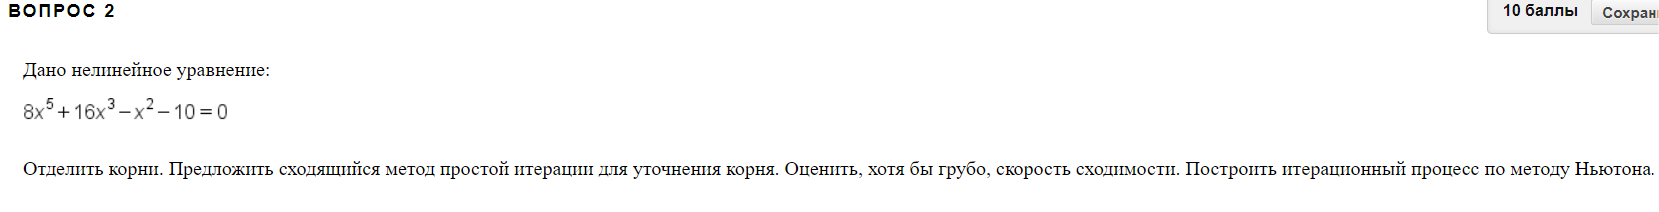
\includegraphics[width=1\textwidth]{last-kr-2.png}
    \label{fig:my_label}
\end{figure}
\section*{Задание №2}

1. Отделение корней
Для нахождения приближенных значений корней проведем анализ функции:
\[ f(x) = 8x^5 + 16x^3 - x^2 - 10 \]
Исследуем функцию на промежутке, чтобы найти изменение знака:
\[-  f(0) = -10 
-  f(1) = 8(1)^5 + 16(1)^3 - (1)^2 - 10 = 13 
\]
Следовательно, корень находится в промежутке \([0, 1]\).
2. Метод простой итерации
Выразим \( x \) через \( x \):
\[ x = g(x) = \sqrt[5]{\frac{10 + x^2 - 16x^3}{8}} \]
3. Итерационный процесс
Начальное приближение \( x_0 = 0.5 \):
\[
x_{k+1} = \sqrt[5]{\frac{10 + x_k^2 - 16x_k^3}{8}}
\]
4. Скорость сходимости
Для грубой оценки скорости сходимости проверим производную \( g'(x) \):
\[
g'(x) = \frac{d}{dx}\left(\sqrt[5]{\frac{10 + x^2 - 16x^3}{8}}\right)
\]
Если \(|g'(x)| < 1\) на отрезке, то метод сходится.
5. Метод Ньютона
Формула метода Ньютона:
\[ x_{k+1} = x_k - \frac{f(x_k)}{f'(x_k)} \]
где
\[ f'(x) = 40x^4 + 48x^2 - 2x \]
Итерационный процесс по методу Ньютона:
\[
x_{k+1} = x_k - \frac{8x_k^5 + 16x_k^3 - x_k^2 - 10}{40x_k^4 + 48x_k^2 - 2x_k}
\]

\end{document}

